\documentclass{report}
\usepackage{fancyhdr} % Required for custom headers
\usepackage{lastpage} % Required to determine the last page for the footer
\usepackage{extramarks} % Required for headers and footers
\usepackage{graphicx} % Required to insert images
%\usepackage{lipsum} % Used for inserting dummy 'Lorem ipsum' text into the template
\usepackage{amsmath}
\usepackage{graphicx} 
\usepackage{float}
%\usepackage{amsfont}
%\usepackage{amssymb}

\usepackage{multicol}
% Margins
\topmargin=-0.5in
\evensidemargin=0in
\oddsidemargin=-0.5in
\textwidth=7.5in
\textheight=9.0in
\headsep=0.25in 


\pagestyle{fancy}

%\rhead{\textbf{Marshall's Recipes}} % Top right header
%\lhead{\textbf{Curry Stir Fry}}
%\chead{ }
%\title{Curry Stir Fry}

\begin{document}
%\vspace{8mm}
%\textbf{PRELIMINARIES:}


\bigskip

\bigskip

\begin{multicols}{2}
\textbf{Ingredients}
\begin{itemize}
\item 1 lb lentils \newline (1690 kCal / 104 gP / 13 gF / 286 gC)
\item 2 cups basmati rice \newline (1280 kCal / 32 gP / 0 gF / 280 gC)
\item 2 yellow onions \quad (90 kCal / 2 gP / 0 gF / 22 gC)
\item 2 cans diced tomatoes \newline (210 kCal / 7 gP / 0 gF / 42 gC)
\item 1 small can tomato sauce \newline (53 kCal / 4 gP / 0 gF / 11 gC)
\item 1 boxes vegetable stock
\item 4 cup water 
\item 6 cloves of garlic
\item 2 tsp. salt
\item 4 tsp. cumin
\item 2 tsp. cayenne pepper
\item 2 tsp. ground ginger
\item 3 tsp. curry powder
\item 3 star anise pods
\item 9 cardamom pods
\item $\frac{1}{2}$ tsp. turmeric 


\end{itemize}


\columnbreak
\textbf{Procedure:}
\medskip


\begin{enumerate}

\item Rinse and drain lentils, then add to pressure cooker. 
\item Add tomatoes, tomato sauce, powdered spices, garlic, water, vegetable stock, and minced onion to pressure cooker. Stir well to ensure that no lentils have stuck to the bottom or have clumped together. 
\item Crush 4 cardamom pods open and add to pressure cooker on the top. 

\item Rinse and drain the rice. Add to a medium pan with three cups of water. Crush the remaining cardamom pods open and add to rice along with star anise. 
\item Bring rice to a boil, put a lid on the pan then reduce heat to low for 15 minutes. 

\item Cook lentils in pressure cooker for 20 minutes or until contents are soft. 
\item Remove cardamom and anise from rice and lentils and discard. Mush the lentils with a utensil before serving over rice. 


\begin{table}[H]
  \begin{center}
    \caption{Macro totals}
    \label{tab:table1}
    \begin{tabular}{c|c|c|c} % <-- Alignments: 1st column left, 2nd middle and 3rd right, with vertical lines in between
      \textbf{Calories} & \textbf{Protein} & \textbf{Fat} & \textbf{Carbs}\\
      \hline
      3323 kCal & 149 g & 13 g & 641 g\\
    \end{tabular}
  \end{center}
\end{table}
 
\end{enumerate}
\end{multicols}




%\begin{center}
%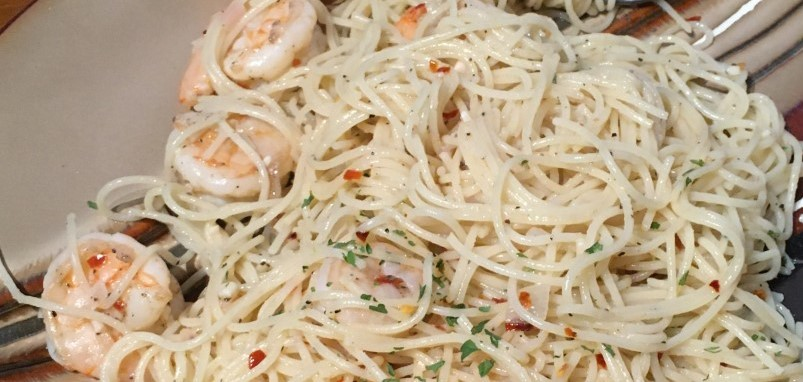
\includegraphics[scale=0.65]{Pasta/Shrimp Scampi/Shrimp Scampi.jpg}
%\end{center}


\end{document}